\documentclass[12pt]{article}
\addtolength{\oddsidemargin}{-.5in}
	\addtolength{\evensidemargin}{-.5in}
	\addtolength{\textwidth}{1in}
	\addtolength{\topmargin}{-.5in}
	\addtolength{\textheight}{.5in}

\usepackage{graphicx}
\begin{document}

\begin{enumerate}
\item {\bf Introduction:}
%
\begin{enumerate}
\item 1.1 Purpose of this Document:\newline
This document will be a detailed analysis of the project I will be working during the summer. 
\item 1.2 Scope of this document:\newline
This document covers the core of the system. It includes the code that will do most of the calculations to find suitable schedules, the GUI for the applet, and the requirements for running the applet.
\item 1.3 Overview:\newline
The program is mainly for college students or those just entering college and need to create a schedule for their classes.  The program will allow students to create effective schedules for their classes without becoming a burden.  Also students will be able to fit their courses around their own day to day schedule, instead of fitting their schedule around their courses.
\item 1.4 Business Context:\newline
The Amp program gives students the chance to experience researching and using resources that are available to them, especially for minorities.  It helps students prepare for graduate school.\newline
\end{enumerate}

\item {\bf General Description:}
\begin{enumerate} 
\item 2.1 Product Functions:\newline
		The system should be able to take in multiple classes with different time slots, create a unique schedule out of every possible combination of classes, then display the schedules that have no conflicting time slots.  The system should also be able to take in other schedules, such as work or any times the student would not like to have class, and determine whether it will conflict with the course schedule.
The system should make it effortless for GMU students to create class schedules that will not interfere with their daily lives.  The system should not jeopardize ease of use for performance.
\item 2.2 Similar System information:\newline
		The product will be used along side a website that will hold the system.  The system will be a web applet. If we can finish the project before the deadline we might be able to turn it into a web application.
\item 2.3 User Characteristics:\newline
		Users do not need prior experience to run the software, but should be familiar with how scheduling works and day to day applications.
\item 2.4 User Problem Statement:\newline
		In order to use the software, users will need to have prepared the classes they would like to schedule which might be difficult.  Users will have to input every single potential timeslot which might become time consuming.
\item 2.5 User Objectives:\newline
		Users will want an easy and fast way to input their courses and the individual timeslots.  Inputting so many different timeslots can become very tedious, so the GUI would need to lessen this task.
We can do this by asking for the class name once, then create textboxes for the users to input different times.  A combo box might be best for the minutes.
Finally the schedule should be displayed in a manner that is easy to read and comprehend.  Somewhat like a calendar.
\item 2.6 General Constraints:\newline
		Since the program will be a web applet it will not have access to system resources, so we cannot save files or run programs on the user�s computer.  We will also need to make the program reusable incase we want to turn it into a stand alone application or a web application.\newline
\end{enumerate}

\item {\bf Functional Requirements:}
\begin{enumerate}
\item System must be able to compute working schedules efficiently and in a timely manner.
		\begin{enumerate} 
		\item Description:\newline
			The applet should not take long to load the working schedules and display them to the user.
		\item Criticality:\newline
			Very critical
		\item Technical issues:\newline
			System will have to not only compare each course but also its labs.  It will also have to compare the final schedules with other the timeslots the student would not like to have class.
		\item Risks:\newline
			If the user inputs wrong data, such as replacing the start time of a course with its end time, the system will not be able to process it.
		\end{enumerate}
		
\item System should be able to store the data temporarily.
		\begin{enumerate} 
		\item Description:\newline
			If the user wants to go back and enter another class or change a timeslot, he should not have to enter all the data in again.  The user should be able to go back to his previous courses easily.
		\item Criticality:\newline
			Very critical.
		\item Technical issues:\newline
			The system will have to somehow display the current courses and timeslots in a way that is easy for the user to read and change.
		\item Risks:\newline
			none\newline
		\end{enumerate}

\item GUI should display the final results in a manner that is readable.
		\begin{enumerate}
		\item Description:\newline
			After the program calculates the working schedules, it should display a chart containing a schedule.  As the user looks through the schedules the chart should redisplay the current schedule that the user is looking at.\newline
			The chart that is displayed should highlight the classes and the times that the user listed as not wanted.
		\item Criticality:\newline
			Very Critical.
		\item Technical issues:\newline
			I am very bad with GUI designs.
		\item Risks:\newline
			Fitting the chart with a schedule that has a lot of classes, in a predetermined size box.
		\end{enumerate}

\item The program should ask for classes that are optional for the student.
		\begin{enumerate}
		\item Description:\newline
			Some classes students are not sure whether they should take them or not depending on their schedule.  The system should show any schedule that contains or does not contain the optional classes.
		\item Criticality:\newline
			Somewhat critical.
		\item Technical issues:\newline
			Applet should have a check box, that users can check if the class is optional.
		\item Risks:\newline
			If there are too many optional classes it will greatly increase the time it takes to calculate the resulting schedules.\newline
		\end{enumerate}
\end{enumerate}
			
\item {\bf Interface Requirements:}
	\begin{enumerate}
	\item 4.1 User Interfaces:\newline
		The system will interface with the user mainly through the GUI.
	\item 4.1.1 GUI:
		\begin{itemize}
		\item The graphical user interface will first present the user with a couple of text boxes and combo boxes for the user to input the class name and its timeslots.  It will also have 4 buttons, NEXT, PREVIOUS, REMOVE, and ADD, which will add that class to the list.
			\begin{itemize}
			\item This will also contain check boxes next to the classes.  The user can check these if the class is optional. 
			\item It will also have a PANEL that displays the classes that were added.  The user can click on any of these to highlight a class, and change its properties.
			\end{itemize}
		\item The next phase, the GUI will present the user with similar boxes for the user to input when he would not be available for classes. 
			This phase might have a chart that the user can use to enter when he is unavailable instead of textboxes.
		\item The third phase, will display the resulting schedule to the student.  It will have a PREVIOUS button incase the student wants to change any class.
		\end{itemize}
	\item 4.1.2 API:\newline
		To be filled later.\newline
	\end{enumerate}

\item {\bf Performance Requirements:}\newline
	Since the system will be an applet the user will only need an internet connection.  If we make it a stand alone application, then the user will need a java virtual machine.\newline

\item {\bf Design Constraints:}
	\begin{itemize}
	\item If the system will save user�s schedules for later use, the information cannot be shown to any other users.
	\item If user is to be asked for any personal information, the system will need a way to obtain proof of the user's permission.
	\item System does not have access to the user's computer so it will need some other way of storing the user's information and previous schedules.  We can do this by using a database or asking the user if he would like to save or download his current work.
	\end{itemize}

\item {\bf Other Non-Functional Attributes:}
	\begin{enumerate}
	\item Security will not be a major issue, unless we will be keeping a database of all the users and their saved work.  That will not be covered by this SRS.
	\item Reliability will be a great issue in the system, mainly because many students will be using it to schedule their classes and small mistakes can greatly effect a student's standing.\newline
	System must be able to keep track of the user's progress, incase an error occurs.
	\item System should also be extensible since it will probably go through a lot of changes.  Features and updates should be easy to setup, without having to change to much in the code.
	\end{enumerate}
	
\item {\bf Premiliminary Object-Oriented Domain Analysis:}
	\begin{enumerate}
	\item Inheritance Relationships:
		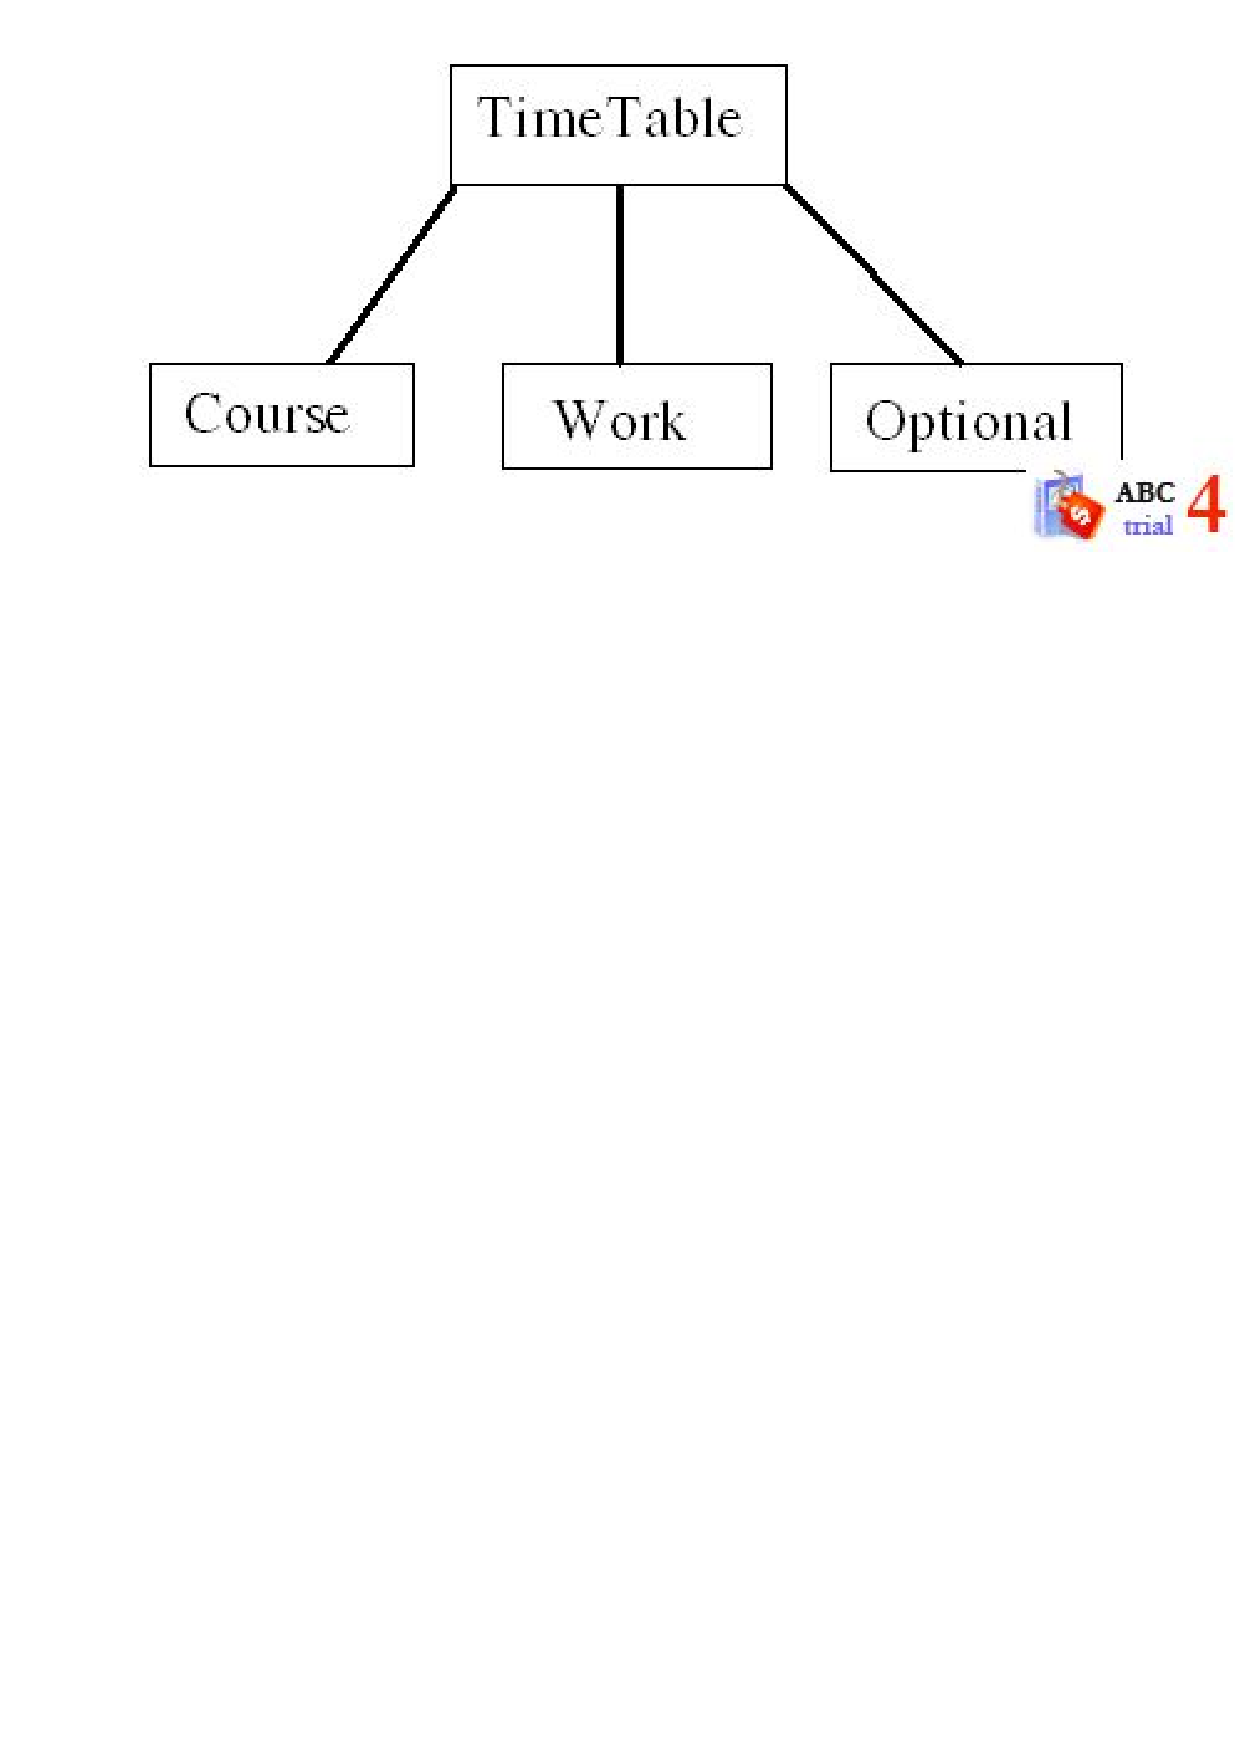
\includegraphics[scale=.40, width=60mm, height=80mm]{graph}
	\item Class Descriptions:
		\begin{enumerate}
		\item {\it CLASS NAME:} TimeTable
			\begin{enumerate}
			\item Abstract
				\begin{itemize}
				\item Course
				\item Work
				\item Optional
				\end{itemize}
			\item {\it PURPOSE:} Abstract class that will contain time tables of different time objects, such as the classes.  This will hold most accessors and modifiers for any objects that will hold a time slot.
			\item {\it ATTRIBUTES:}
				\begin{itemize}
				\item String name
				\item int startTime, {\bf range:} 0 \- 2400.
				\item int endTime, {\bf range:} 0 \- 2400.
				\end{itemize}
			\end{enumerate}
		\end{enumerate}
	\end{enumerate}

\item {\bf Operational Scenarios:}	
	\begin{itemize}
	\item The user would start the applet and the GUI displayed will contain 2 text boxes.  User would enter the name of the first class in the first box and the class section in the second box.  He would then have an empty table, this is where his time slots would be shown.  Above that is an area with two boxes, he can enter the first time slot then click add.  That time would be added to the table and the two boxes would be cleared.  There will be a check box for the user to check if that time slot is optional for him.  He would do this until he input all the times.  Then he would click the next button which would clear all the boxes and start over. Finally when he has input all his courses he will click finish, this displays a panel that has somwhat the same layout as the one before but instead asks for times that the user does not want to have class.  When he is done he will click finish. The GUI will then display a table, resembling a calendar or planner.  After it has calculated the working schedules, it will display it in the table.  The classes he wants will be highlighted.  He can then go back to change something or click FINISH.
	\end{itemize}
\end{enumerate}

\end{document}
